\begin{figure}[h]
    \centering
    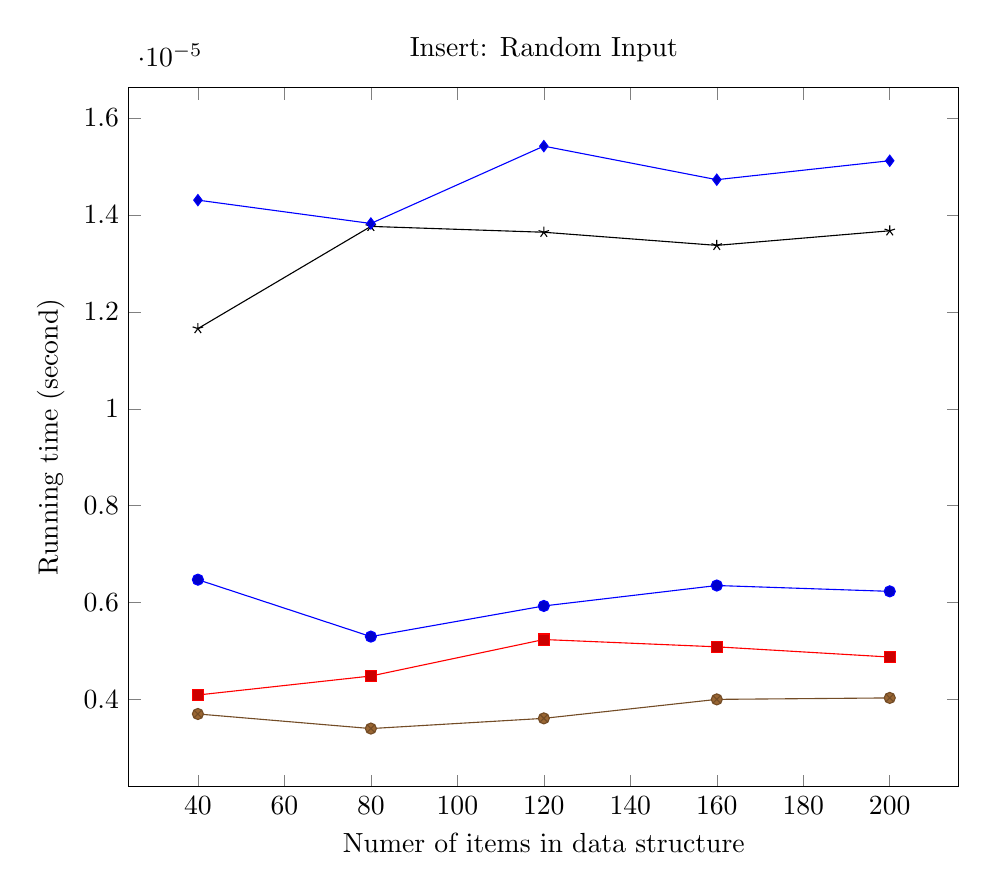
\begin{tikzpicture}
        \begin{axis}[
            xlabel={Numer of items in data structure},
            ylabel={Running time (second)},
            title={Insert: Random Input},
            width=\textwidth
        ]
		\addplot coordinates {
			(200, 6.234329470800048e-06)
			(160, 6.354799605290396e-06)
			(120, 5.933154134041274e-06)
			(80, 5.300685926812321e-06)
			(40, 6.475269740136014e-06)
		};
		\addplot coordinates {
			(200, 4.879040455207928e-06)
			(160, 5.089863190832488e-06)
			(120, 5.240450859389511e-06)
			(80, 4.487512517670212e-06)
			(40, 4.095984579777223e-06)
		};
		\addplot coordinates {
			(200, 4.035749512354414e-06)
			(160, 4.005631978998281e-06)
			(120, 3.6141040411052925e-06)
			(80, 3.4032813054807322e-06)
			(40, 3.704456641884235e-06)
		};
		\addplot coordinates {
			(200, 1.3673360288635195e-05)
			(160, 1.337218495187642e-05)
			(120, 1.364324275492379e-05)
			(80, 1.3763712889414137e-05)
			(40, 1.1655485532102716e-05)
		};
		\addplot coordinates {
			(200, 1.5119001905006257e-05)
			(160, 1.472747396711327e-05)
			(120, 1.5420177241765032e-05)
			(80, 1.3823947956836945e-05)
			(40, 1.4305828495508876e-05)
		};
        \legend{}
        \end{axis}
    \end{tikzpicture}
    \caption{Average of 0 operations, benchmarked every 0, starting at 0.}
\end{figure}